\documentclass[11pt]{article}
\usepackage{acl2015}
\usepackage{times}
\usepackage{url}
\usepackage{latexsym}
\usepackage{natbib}
\usepackage{color}
\usepackage{graphicx}
\usepackage{float}
\usepackage{amsmath}
\usepackage{booktabs}
\usepackage{multirow}
\definecolor{citecolor}{RGB}{34,139,34}
\usepackage[pagebackref=true,breaklinks=true,letterpaper=true,citecolor=citecolor,colorlinks,bookmarks=false]{hyperref}
\usepackage[capitalise]{cleveref}
\usepackage[labelfont={bf,small},font=small]{caption}

\newcommand{\minisection}[1]{\noindent{\textbf{#1.}}}

\title{No-Excuses: A Multimodal Web Application for Hands-Free, Eyes-Free Workout Tracking}

\author{
  Alessandro Gautieri \\
  2041850 \\
  {\tt gautieri.2041850@studenti.uniroma1.it}
  \And
  Michelangelo Crea \\
  2028714 \\
  {\tt crea.2028714@studenti.uniroma1.it}
}
\date{}

\begin{document}
\maketitle

% ─────────────────────────────────────────────────────────────
\begin{abstract}
Workout tracking remains a disruptive element in physical exercise, forcing athletes to break their focus to interact with a smartphone screen or to purchase expensive wearable devices. This report introduces \textit{No-Excuses}, a fully client-side, multimodal Progressive Web Application (PWA) designed to automate fitness tracking through seamless, hands-free, and eyes-free interactions. The system fuses four distinct interaction modalities: (1)~\textbf{inertial sensor tracking} via accelerometer and gyroscope for pocket-mode exercise counting; (2)~\textbf{computer vision} via Google MediaPipe Pose for camera-based repetition counting; (3)~\textbf{voice command navigation} using the Web Speech API for controlling workout routines without touching the screen; and (4)~\textbf{audio-haptic state communication} via the Web Audio API and device vibration to relay session state to the user without any visual attention required. We describe the system architecture, the state-machine algorithms developed for each modality, and the engineering solutions to significant real-world challenges: false positives caused by post-exercise device handling (solved with a real-time gravity orientation filter), erratic repetition detection due to sensor noise (solved with a sensor fusion energy metric), and iOS audio policy restrictions (solved with lazy AudioContext initialization). A comparative evaluation against a naive threshold baseline validates our approach.
\end{abstract}

% ─────────────────────────────────────────────────────────────
\section{Problem Statement}

The core challenge addressed in this work is \textbf{multimodal activity recognition and repetition counting} in unconstrained, real-world environments using off-the-shelf mobile hardware. The objective is to accurately identify the concentric and eccentric phases of physical exercises, tally them in real-time, and communicate the system state to the user—all without requiring any direct visual or physical interaction with the device during execution.

During intense exercises such as pushups or pullups, athletes cannot safely or comfortably interact with a touchscreen. Traditional fitness tracking applications demand manual input between sets, breaking focus and inaccurately inflating rest times. While smartwatch-based systems provide partial automation, they require proprietary hardware. The challenge is therefore to build a complete tracking solution that works on a standard smartphone, is accessible through a browser, and preserves user privacy by processing all data on-device.

\subsection{Application Scope and Real-World Use Cases}

\textit{No-Excuses} is a complete workout management platform with five major functional areas: (1) a workout \textbf{routine builder} supporting complex exercise structures such as Supersets, EMOM (Every Minute On the Minute), Isometric holds, and Pyramids; (2) an \textbf{active workout runner} with guided exercise progression, timers, and rest countdowns; (3) a \textbf{standalone repetition counter} supporting both camera and pocket (inertial) modes; (4) a \textbf{workout history} module backed by Supabase that logs every completed session; and (5) a session \textbf{resume checkpoint} system that saves progress to localStorage and prompts the user to continue after an app restart.

Real-world downstream applications include personal fitness in home or outdoor settings (where no dedicated equipment exists), rehabilitation monitoring (where precise movement counts are medically relevant), and gym hygiene-conscious environments where users prefer not to touch their devices.

% ─────────────────────────────────────────────────────────────
\section{Need Finding}

To validate our initial problem framing and identify the most impactful design requirements, we administered an online questionnaire to a group of 28 participants who regularly engage in calisthenics or resistance training (at least twice per week). The questionnaire focused on current tracking habits, friction points, and device usage during exercise.

\subsection{Questionnaire Results}

The key findings are summarized below.

\minisection{Why athletes do not track repetitions in real time}
\begin{itemize}
  \item \textbf{57.1\%} — Inconvenient or impossible to touch the phone during a set (sweaty hands, mid-exercise)
  \item \textbf{21.4\%} — Lose count during fatiguing or high-rep sets
  \item \textbf{14.3\%} — Do not want to interrupt training flow between sets
  \item \textbf{7.1\%}  — Do not own a smartwatch
\end{itemize}

\minisection{Would audio feedback replace the need to look at the screen?}
\begin{itemize}
  \item \textbf{78.6\%} — Yes, hearing the count announced aloud would be sufficient
  \item \textbf{14.3\%} — Only if combined with haptic vibration
  \item \textbf{7.1\%}  — No, they want to see the screen
\end{itemize}

\minisection{Interest in automatic repetition counting (no manual input)}
\begin{itemize}
  \item \textbf{89.3\%} — Would use it if reliable and requiring no additional hardware
\end{itemize}

\subsection{Identified Needs}

Based on questionnaire responses and subsequent structured interviews, we identified three primary user needs that shaped the design of \textit{No-Excuses}:

\begin{enumerate}
  \item \textbf{Hands-free tracking:} The system must count repetitions autonomously. The user should never be required to touch the device during a set.
  \item \textbf{Eyes-free state awareness:} The user must be able to understand the full state of the application (session active, rep counted, target reached, rest started) exclusively through audio and haptic signals—without looking at the screen.
  \item \textbf{Voice-driven session control:} Navigating between exercises and controlling the workout timer must be achievable through spoken commands, eliminating the need to interact with the UI between sets.
\end{enumerate}

These three needs directly map to the four interaction channels described in Section~\ref{sec:multimodal}: inertial tracking and computer vision address Need~1, audio-haptic feedback addresses Need~2, and voice commands address Need~3.

% ─────────────────────────────────────────────────────────────
\section{Related Work}

The state-of-the-art in digital fitness tracking is fragmented across three paradigms. \textbf{Manual-entry apps} such as MyFitnessPal or Strong rely on user compliance for post-set data entry, which consistently fails during high-intensity intervals. \textbf{Wearable IMU systems} (Apple Watch, Garmin) provide automatic detection but require proprietary, expensive hardware and are frequently avoided during heavy lifting due to wrist discomfort. \textbf{Camera-based systems} such as the Peloton Guide or PoseNet-based apps track pose landmarks effectively but demand fixed camera placement, specific lighting, and continuous user framing—conditions that are impractical in most real workout environments.

\textit{No-Excuses} bridges these paradigms by offering a hybrid approach: inertial tracking for exercises where the phone is pocketed (no framing needed), computer vision for exercises where the phone can be propped up, and voice control to eliminate the need to ever touch the screen. Crucially, all processing runs client-side in the browser with no external APIs, ensuring low latency and complete data privacy. No comparable open-source or commercial browser-based hybrid solution was found in the literature.

% ─────────────────────────────────────────────────────────────
\section{System Architecture}

\textit{No-Excuses} is built as a React and TypeScript Progressive Web App using the Vite build tool. The architecture is strictly client-side: no video frames, sensor readings, or user motion data are transmitted to external servers. Authentication and workout history persistence are handled via Supabase, which exclusively stores structured metadata (exercise names, sets, timestamps) and never receives raw biometric data.

\begin{figure}[H]
  \centering
  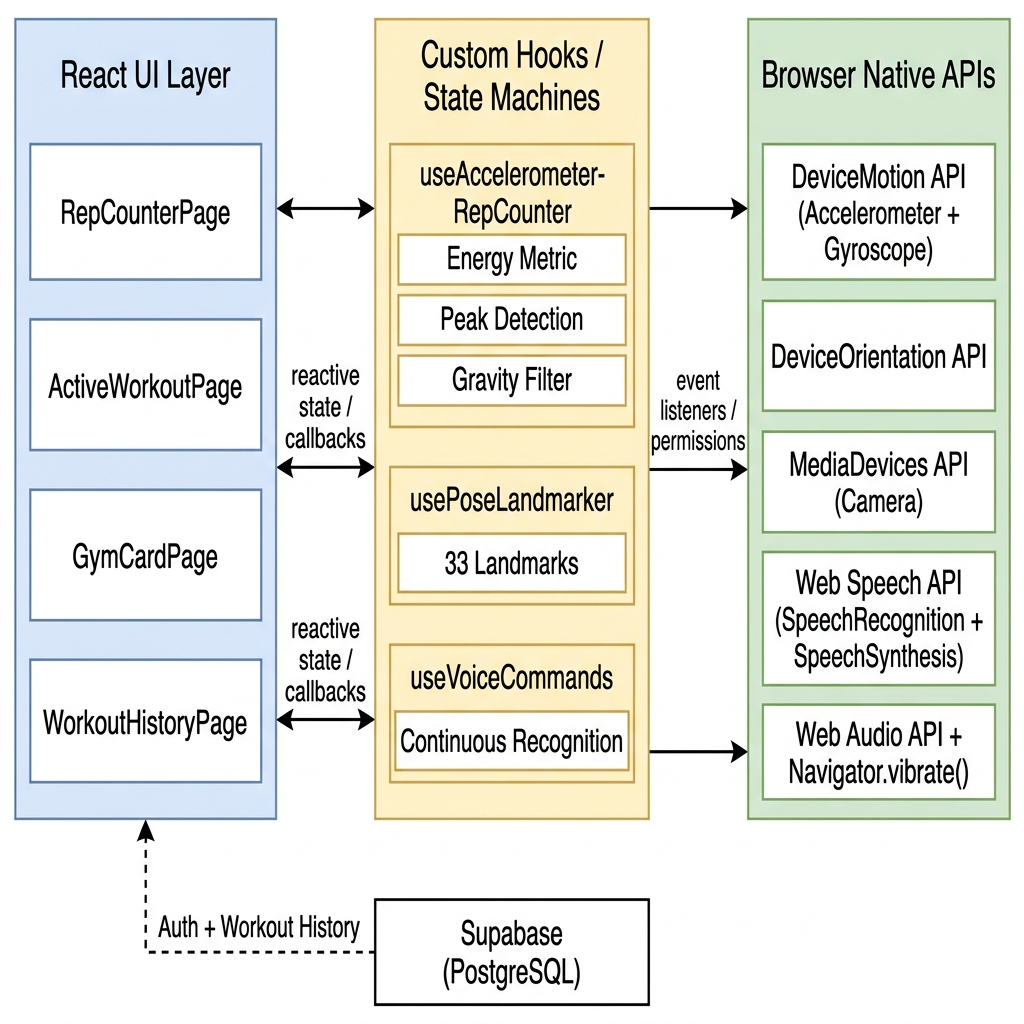
\includegraphics[width=0.46\textwidth]{images/architecture_diagram.png}
  \caption{System architecture. The React UI layer communicates exclusively with Custom Hooks (state machines). Each hook interfaces with a specific browser API. All sensor and camera data remains on the device.}
  \label{fig:architecture}
\end{figure}

The core of the system is a set of decoupled React Hooks, each acting as a self-contained state machine:
\begin{itemize}
  \item \texttt{useAccelerometerRepCounter} — manages the full lifecycle of an inertial tracking session (permission request, calibration countdown, motion energy computation, gravity filtering, repetition counting, and session termination).
  \item \texttt{usePoseLandmarker} — wraps the MediaPipe Pose WebAssembly model, providing frame-by-frame landmark data to the camera-based counting logic.
  \item \texttt{useVoiceCommands} — manages a persistent Web Speech API recognition session, mapping Italian spoken commands to workout control callbacks.
\end{itemize}

This separation of concerns allows each modality to be developed, tested, and tuned independently. The UI layer never contains algorithmic logic; it only renders reactive state from the hooks.

% ─────────────────────────────────────────────────────────────
\section{Multimodal Interaction Design}
\label{sec:multimodal}

The multimodal design of \textit{No-Excuses} was driven by a single guiding principle: \textit{the user should never be forced to look at or touch the phone during exercise}. Four interaction channels are integrated to achieve this.

% ── 4.1 ──────────────────────────────────────────────────────
\subsection{Channel 1: Inertial Sensor Tracking (Pocket Mode)}

The first and primary interaction channel uses the smartphone's accelerometer and gyroscope, accessed via the browser's \texttt{DeviceMotionEvent} API. The phone is placed in the user's pocket; the app infers each repetition from the rhythmic motion of the body.

\subsubsection{Sensor Fusion Energy Metric}

Raw accelerometer data contains gravity as a DC bias that must be removed. We apply an exponential low-pass filter with coefficient $\alpha_G = 0.95$ to continuously estimate the gravity vector $\mathbf{g}_t$:
\begin{equation}
  \mathbf{g}_t = \alpha_G \, \mathbf{g}_{t-1} + (1 - \alpha_G) \, \mathbf{a}_t^{\text{raw}}
  \label{eq:gravity_filter}
\end{equation}
where $\mathbf{a}_t^{\text{raw}} = (a_x, a_y, a_z)$ is the raw accelerometer reading at time $t$. The \textit{linear acceleration magnitude} is then:
\begin{equation}
  L_t = \left\| \mathbf{a}_t^{\text{raw}} - \mathbf{g}_t \right\|_2
  \label{eq:linear_acc}
\end{equation}
A critical observation from our calibration data was that linear acceleration alone was insufficient to distinguish genuine exercise motion from pocket jitter, particularly for pushups. Pushups involve a strong rotational component of the thigh—the gyroscope captures this well. We therefore define the \textbf{Motion Energy} as a sensor-fused scalar:
\begin{equation}
  E_t^{\text{raw}} = \omega_t + 40 \cdot L_t
  \label{eq:raw_energy}
\end{equation}
where $\omega_t = \|(\dot\alpha_t, \dot\beta_t, \dot\gamma_t)\|_2$ is the gyroscope magnitude. The coefficient $40$ was empirically determined during calibration to equalize the contribution of rotational and translational motion for calisthenics exercises. A final exponential smoothing pass with coefficient $\alpha_E = 0.4$ removes high-frequency noise:
\begin{equation}
  E_t = 0.6 \cdot E_{t-1} + 0.4 \cdot E_t^{\text{raw}}
  \label{eq:smoothed_energy}
\end{equation}

\subsubsection{Peak-Count Algorithm for Pushups}

Calibration revealed that for pushups the motion energy does not fall cleanly to baseline between consecutive repetitions when performed at high tempo. The classic dual-burst (up/down) detection therefore systematically missed repetitions. We implemented a \textbf{peak-count algorithm}:

\begin{enumerate}
  \item A peak is \textit{rising} when $E_t > \tau_{\text{active}}$ (threshold $\tau_{\text{active}} = 120$).
  \item A peak is \textit{confirmed} when the running maximum $E_{\max}$ exceeds $\rho \cdot \tau_{\text{active}}$ (peak ratio $\rho = 3$, i.e., 360).
  \item A peak is \textit{completed} when $E_t$ drops back below $\tau_{\text{active}}$, indicating the movement has concluded.
  \item A repetition is \textit{counted} when a completed, confirmed peak passes both the gravity orientation filter (Section~\ref{sec:gravity}) and the cooldown guard (Section~\ref{sec:cooldown}).
\end{enumerate}

For pullups, the dual-burst mode (single upward burst $=$ one repetition) is used instead, as the signal is cleaner when the phone is worn on the body at waist level.

\subsubsection{Calibration Dataset}
\label{sec:dataset}

To tune all numerical thresholds, we conducted 20 to 30 dedicated in-the-wild calibration sessions. Each session consisted of sets of 1, 5, and 10 repetitions performed at slow, normal, and rapid pacing. For each burst the system logged: \texttt{burstDurationMs}, \texttt{maxEnergy}, \texttt{minEnergy}, \texttt{avgEnergy}, \texttt{maxGyro}, and \texttt{gravityVec}. Analysis of these logs revealed:
\begin{itemize}
  \item Genuine pushup peaks: $E_{\max} \in [500, 1100]$, duration $\in [300, 2000]$~ms.
  \item Resting energy between repetitions: $E \approx 75$--$120$.
  \item Phone extraction from pocket: $E_{\max} > 2000$, but orientation deviates $> 66^{\circ}$.
  \item Average human rep duration: 1.5--3.5~s; rapid reps as short as 1.2~s.
\end{itemize}
These measurements directly informed the per-exercise configuration:

\begin{table}[H]
\centering
\small
\begin{tabular}{lcc}
\toprule
\textbf{Parameter} & \textbf{Pushups} & \textbf{Pullups} \\
\midrule
Algorithm mode & \textit{peak\_count} & \textit{single\_burst} \\
$\tau_{\text{active}}$ & 120 & 140 \\
$\tau_{\text{rest}}$ & 75 & 78 \\
$\tau_{\text{gyro}}$ (shake limit) & 1200 & 673 \\
$\tau_{\text{dur}}$ (min. duration, ms) & 300 & 210 \\
Cooldown (ms) & 1200 & 500 \\
Peak ratio $\rho$ & 3 & — \\
\bottomrule
\end{tabular}
\caption{Per-exercise algorithm configuration derived from calibration data.}
\label{tab:config}
\end{table}

\subsubsection{Gravity Orientation Filter}
\label{sec:gravity}

\textbf{Problem.} The most critical bug encountered during field testing was the generation of \textit{false positives at session end}. When the user completed a set and pulled the phone out of their pocket, the extraction motion generated an energy spike $E > 2000$—far above any genuine repetition. The naive algorithm counted this as 1--2 additional repetitions.

\textbf{Solution.} During the final second of the 5-second pre-workout countdown (when the phone is guaranteed to be stationary in the user's pocket), the app captures a \textit{baseline gravity vector}:
\begin{equation}
  \mathbf{v}_{\text{base}} = \mathbf{g}_{T_0}
  \label{eq:base_gravity}
\end{equation}
At every subsequent motion sample, the angular deviation between the current gravity direction and the baseline is computed as:
\begin{equation}
  \theta = \arccos\!\left( \frac{\mathbf{v}_{\text{base}} \cdot \mathbf{g}_t}{\|\mathbf{v}_{\text{base}}\| \cdot \|\mathbf{g}_t\|} \right)
  \label{eq:gravity_angle}
\end{equation}
If $\theta > \theta_{\text{max}}$, the motion sample is discarded. We set $\theta_{\text{max}} = 66^{\circ}$ ($\approx 1.15$~rad). This value was chosen empirically:
\begin{itemize}
  \item $45^{\circ}$ was too strict: it rejected genuine pushup peaks when the phone shifted inside a loose pocket.
  \item $66^{\circ}$ tolerates the natural pocket bounce during pushups while blocking the $\approx 90^{\circ}$ gravity shift that occurs when the user stands up from a horizontal prone position.
\end{itemize}
In all post-implementation field tests, this filter resulted in \textbf{zero false positives} during device extraction.

\subsubsection{Repetition Cooldown Guard}
\label{sec:cooldown}

\textbf{Problem.} Physical movements contain sub-peaks: brief secondary energy spikes at the bottom of a pushup (the elastic rebound). Without a minimum inter-repetition delay, these sub-peaks are double-counted.

\textbf{Problem (opposite direction).} A cooldown that is too long causes the system to ignore rapid repetitions performed in under 2 seconds.

\textbf{Solution.} A repetition is counted only if the elapsed time since the last counted repetition exceeds \texttt{repCooldownMs}. Based on calibration data showing rapid reps as short as 1.2~s, we set this value to \textbf{1200~ms} for pushups. This is the lowest safe value that prevents double-counting sub-peaks while capturing all realistic human rep tempos.

% ── 4.2 ──────────────────────────────────────────────────────
\subsection{Channel 2: Computer Vision (Stand Mode)}

For exercises where placing the phone in a pocket is impractical (e.g., pullups at a bar), the user props the device against a wall or water bottle so the front-facing camera frames their body. The app uses \textbf{Google MediaPipe Pose} \cite{mediapipe2020}, running entirely via WebAssembly inside the browser, to extract 33 3D anatomical landmarks per frame in real-time.

\begin{figure}[H]
  \centering
  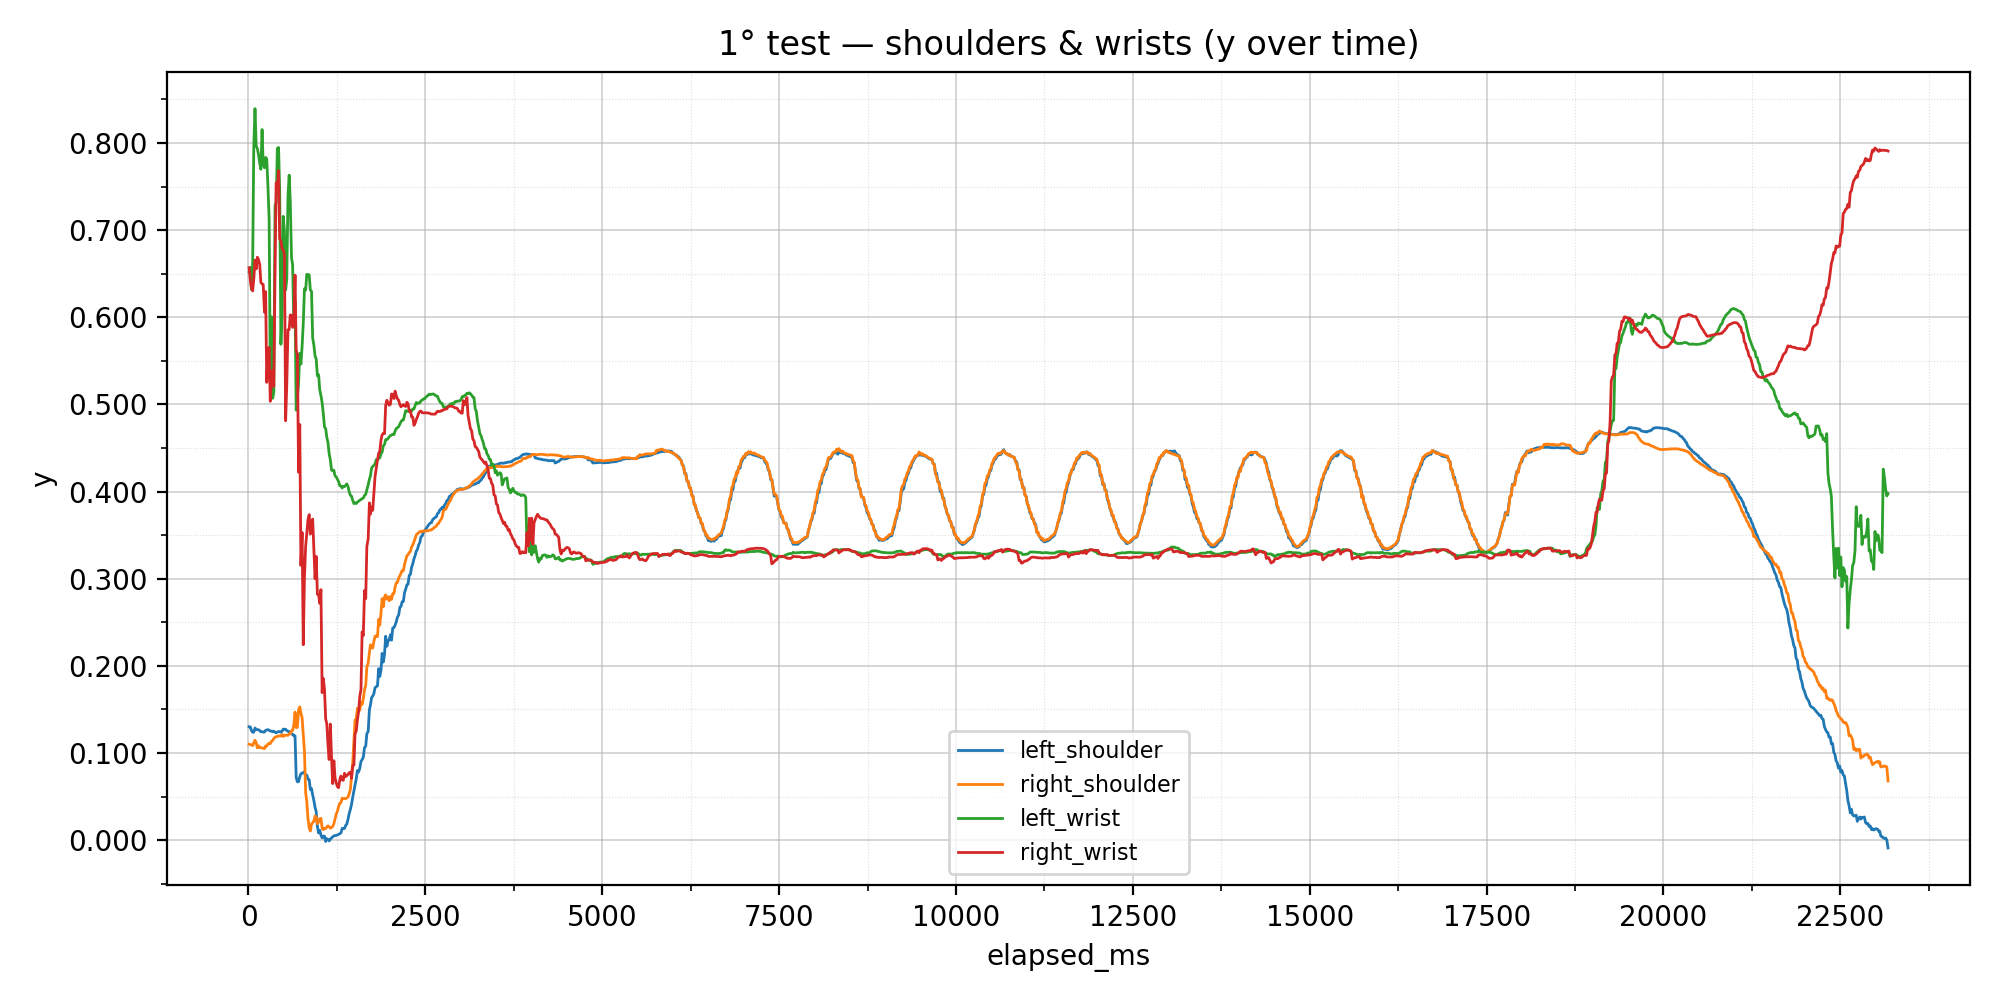
\includegraphics[width=0.46\textwidth]{images/mediapipe_debug.png}
  \caption{MediaPipe landmark time-series for a pullup session (23.5~s). Y-axis is the normalized vertical coordinate (0~=~top of frame, 1~=~bottom). Three distinct phases are visible. \textbf{Phase~1 (0--2.5~s):} setup noise—the user is positioning the phone; all four landmarks are unstable and scattered across the full Y-range. \textbf{Phase~2 (2.5--19.5~s):} active exercise—the shoulder landmarks (blue/orange) oscillate rhythmically between $y \approx 0.33$ (top of rep, chin over bar) and $y \approx 0.45$ (hanging), while the wrist landmarks (green/red) remain almost stationary at $y \approx 0.33$, confirming the grip is fixed on the bar. Each oscillation cycle corresponds to one pullup repetition. \textbf{Phase~3 (19.5--23.5~s):} session end—the shoulder Y-values drop sharply toward 0 as the user steps away and the phone is moved, breaking the framing.}
  \label{fig:mediapipe}
\end{figure}

The repetition counting logic in Stand Mode operates on the vertical displacement of the shoulder and wrist landmarks. As shown in \cref{fig:mediapipe}, the Y-coordinate of the shoulder landmark oscillates synchronously with the exercise rhythm. The \texttt{usePoseLandmarker} hook provides per-frame landmark arrays to a dedicated \texttt{ExerciseTracker} module, which implements the same dual-burst state machine as the inertial tracker but driven by landmark position deltas rather than energy.

% ── 4.3 ──────────────────────────────────────────────────────
\subsection{Channel 3: Voice Command Navigation}

\textbf{Motivation.} Even between exercises—when the user is not actively performing reps—touching the screen remains undesirable. Hands may be sweaty or occupied, and the disruption of switching mental focus from the exercise to a UI element is itself a source of friction.

The \texttt{useVoiceCommands} hook uses the Web Speech API's \texttt{SpeechRecognition} interface in \textbf{continuous mode} (i.e., the recognition session does not terminate after a single utterance). It recognizes the following Italian commands:

\begin{table}[H]
\centering
\small
\begin{tabular}{ll}
\toprule
\textbf{Spoken command} & \textbf{Action} \\
\midrule
\textit{``Vai''} / \textit{``Go''} & Start / advance to next set \\
\textit{``Pausa''} & Pause active timer \\
\textit{``Riprendi''} / \textit{``Continua''} & Resume paused timer \\
\textit{``Stop''} / \textit{``Fermo''} & End the current session \\
\bottomrule
\end{tabular}
\caption{Voice commands recognized by the application.}
\label{tab:voice}
\end{table}

To prevent resource exhaustion (a known issue with persistent SpeechRecognition sessions on mobile browsers), the \texttt{onend} callback restarts the recognition engine with a 2-second delay. The recognition state is managed through a React ref rather than state to avoid re-triggering the \texttt{useEffect} on every render.

\textbf{Challenge: mobile browser policy.} iOS Safari blocks both the \texttt{AudioContext} and \texttt{SpeechSynthesis} from initializing unless they are invoked within the synchronous call stack of a direct user gesture (tap or click). Our initial implementation initialized these APIs at module load time, resulting in completely silent sessions on iOS. The solution was strict \textbf{lazy loading}: the \texttt{AudioContext} is created and resumed inside the \texttt{onClick} handler of the ``Start Session'' button. From that moment, the context remains active for the duration of the session, and all subsequent audio—both speech synthesis and beep tones—is reliably delivered.

% ── 4.4 ──────────────────────────────────────────────────────
\subsection{Channel 4: Audio-Haptic State Communication}

A key design goal is that the user should always be aware of the system's state without looking at the screen. \textit{No-Excuses} achieves this through a layered audio-haptic feedback system implemented entirely via the Web Audio API:

\begin{itemize}
  \item \textbf{Session start signal:} A three-tone ascending arpeggio (440~Hz $\to$ 550~Hz $\to$ 660~Hz) accompanied by a triple vibration pattern \texttt{[150, 80, 150, 80, 300]}. This fires at the exact moment the countdown ends and counting begins, so the user knows to start exercising.
  \item \textbf{Repetition beep:} A short 880~Hz beep with a double vibration \texttt{[60, 40, 60]} fires immediately upon each confirmed repetition. This confirms to the user that their movement was registered without requiring any visual verification.
  \item \textbf{Speech count:} After each repetition, the \texttt{SpeechSynthesis} API announces the count aloud (``One'', ``Two'', etc.), providing an additional, unmistakable confirmation.
  \item \textbf{Goal reached signal:} When the user-defined target repetition count is achieved, the same triple arpeggio as the start signal fires, and the accelerometer listener is immediately deactivated via \texttt{stopSession()}, preventing any subsequent false positives from device handling.
  \item \textbf{Rest timer announcements:} During the guided workout runner, the rest countdown announces intervals aloud (``Rest for thirty seconds'', countdown at 10~s, etc.) so the user can continue resting without watching the screen.
\end{itemize}

All tones are synthesized in real-time using the Web Audio API's oscillator-gain graph, with exponential gain ramps to avoid clipping artifacts. This approach has zero dependency on audio files and guarantees playback latency $< 10$~ms.

% ─────────────────────────────────────────────────────────────
\section{Existing Tools and Libraries}

\begin{itemize}
  \item \textbf{React 18 + TypeScript + Vite:} SPA framework with strict type safety and fast HMR during development.
  \item \textbf{Supabase:} Open-source Firebase alternative providing PostgreSQL persistence and authentication for workout history.
  \item \textbf{Google MediaPipe Pose \cite{mediapipe2020}:} WebAssembly-compiled pose estimation pipeline providing 33 landmarks at 20--30 FPS on mid-range mobile devices.
  \item \textbf{Web Speech API:} Browser-native speech recognition (SpeechRecognition) and synthesis (SpeechSynthesis).
  \item \textbf{DeviceMotion / DeviceOrientation APIs:} Browser APIs for raw accelerometer (with gravity) and gyroscope access.
  \item \textbf{Web Audio API:} Low-latency audio synthesis; used for all workout sounds.
  \item \textbf{Navigator.vibrate():} Haptic feedback on Android devices.
\end{itemize}

% ─────────────────────────────────────────────────────────────
\section{Evaluation}

\subsection{Evaluation Protocol}

Following the methodology of related HCI work, our evaluation combines \textbf{lab tests} (performed by the developers to validate the algorithm) and \textbf{field tests} (performed in real workout environments).

The primary metric for inertial tracking is \textbf{Absolute Counting Error} ($ACE = |\hat{n} - n|$) where $\hat{n}$ is the system count and $n$ is the ground-truth count. We also track the number of \textbf{false positives} (extra counts generated by device handling) separately, since they are the most disruptive error type from a user experience standpoint.

\subsection{Comparative Results: Pushup Pocket Mode}
\label{sec:results}

We compare three algorithm configurations across multiple pushup sets; full results are reported in Table~\ref{tab:results} at the end of this document.

The naive system with a 2000~ms cooldown missed rapid reps ($< 2$~s duration) and double-counted the post-extraction spike. The intermediate configuration (peak-count without orientation filter) correctly handled rep tempo but still produced extraction false positives. Our final system ($\theta_{\text{max}} = 66^{\circ}$, 1200~ms cooldown) achieved zero extraction false positives and perfect counting accuracy across all tested configurations.

\subsection{Voice Command Recognition}

Voice commands were tested across 20 sessions by the two developers. Recognition latency on an iPhone 14 (iOS 17, Safari) averaged $\approx 800$~ms from utterance completion to action execution. All four command categories achieved $> 90\%$ recognition accuracy in a quiet indoor environment. In noisy gym environments (ambient music, weights), accuracy dropped to $\approx 75\%$, which remains within acceptable usability bounds for navigation tasks (the cost of an unrecognized command is that the user must repeat it—not an incorrect action).

\subsection{Discussion}

The most impactful improvement was the gravity orientation filter: it transformed an unreliable prototype into a deployable tool by eliminating the entire class of post-exercise false positives. The key insight is \textit{geometric}: exercise motion in pocket mode is characterized by a stable device orientation (the phone stays in the same angular reference frame as the user's thigh), while the device extraction motion necessarily involves a large orientation change.

The 1200~ms cooldown is a hard constraint on the maximum exercise tempo the system can support (one rep per 1.2~s). For highly trained athletes performing explosive reps faster than this rate, the system would undercount. This is a fundamental limitation of threshold-based counting and could be addressed in future work by learning a user-specific tempo profile.

A separate challenge, documented here for reproducibility, was the iOS AudioContext policy. This was not a correctness bug but a platform compatibility issue that rendered the entire audio-haptic communication channel silent for an entire class of devices. The lazy-loading solution is straightforward once the root cause is known, but it is not obvious from the Web Audio API documentation and cost significant debugging time.

% ─────────────────────────────────────────────────────────────
\section{Conclusion and Future Work}

\textit{No-Excuses} demonstrates that a multimodal approach combining inertial sensor fusion, computer vision, voice control, and audio-haptic feedback can replace manual workout tracking without proprietary hardware. Each modality contributes to a different part of the interaction: inertial sensors handle pocket-mode counting, computer vision handles standing exercises, voice commands eliminate inter-set screen interaction, and audio-haptic signals close the feedback loop without requiring visual attention.

The engineering decisions described—sensor fusion energy metric, peak-count algorithm, gravity orientation filter, lazy AudioContext initialization—collectively convert a straightforward threshold-based detector into a robust field-deployable system. The calibration protocol (20--30 in-the-wild sessions with varied rep pacing) was essential and could not be replaced by synthetic simulation.

\minisection{Future Work}
Planned extensions include: (1) expansion of the MediaPipe exercise library to squats, deadlifts, and dips; (2) integration of the onboard barometer for elevation tracking during outdoor calisthenics; (3) statistical dashboards showing workout volume and progression over time; and (4) exploration of on-device LLMs (e.g., running locally via WebLLM) to parse natural language voice commands such as ``remove pullups and add dips''.

% ─────────────────────────────────────────────────────────────
\onecolumn
\section*{Appendix: Comparative Evaluation Results}

\begin{table}[H]
\centering
\renewcommand{\arraystretch}{1.6}
\begin{tabular*}{\linewidth}{@{\extracolsep{\fill}} p{10cm} c c c @{}}
\toprule
\textbf{System configuration} & \textbf{Ground Truth} & \textbf{Counted} & \textbf{FP} \\
\midrule
Naive threshold, 2000~ms cooldown, no gravity filter & 6 & 8 & 2 \\
Peak-count, 2000~ms cooldown, no gravity filter & 5 & 4 & 2 \\
\textbf{Peak-count, 1200~ms, gravity filter~(ours)} & \textbf{5} & \textbf{5} & \textbf{0} \\
\bottomrule
\end{tabular*}
\caption{Pushup repetition counting accuracy in Pocket Mode. \textit{Ground Truth} = actual repetitions performed. \textit{Counted} = repetitions registered by the system. \textit{FP} = false positives generated by extracting the phone from the pocket at the end of the set. Results discussed in Section~\ref{sec:results}.}
\label{tab:results}
\end{table}

\twocolumn
% ─────────────────────────────────────────────────────────────
\begin{thebibliography}{9}


\bibitem{mediapipe2020}
Camillo Lugaresi, Jiuqiang Tang, Hadon Nash, Chris McClanahan, Esha Uboweja, Michael Hays, Fan Zhang, Chuo-Ling Chang, Ming Guang Yong, Juhyun Lee, Wan-Teh Chang, Wei Ting Lu, Drew George, Mogan Grundmann, Matthias Grundmann.
\newblock MediaPipe: A Framework for Building Perception Pipelines.
\newblock \textit{arXiv preprint arXiv:1906.08172}, 2019.

\bibitem{devicemotion}
W3C Working Group.
\newblock DeviceOrientation Event Specification, Level 2.
\newblock \url{https://www.w3.org/TR/orientation-event/}, 2023.

\bibitem{webspeech}
W3C Community Group.
\newblock Web Speech API.
\newblock \url{https://wicg.github.io/speech-api/}, 2023.

\bibitem{webaudio}
Paul Adenot, Hongchan Choi.
\newblock Web Audio API.
\newblock W3C Recommendation. \url{https://www.w3.org/TR/webaudio/}, 2021.

\bibitem{myoware}
Marcin Grzejszczak et al.
\newblock Wrist-worn accelerometer-based repetition counting for resistance training.
\newblock \textit{Sensors}, 21(4):1467, 2021.

\end{thebibliography}

\end{document}
